% This file was created with tikzplotlib v0.10.1.
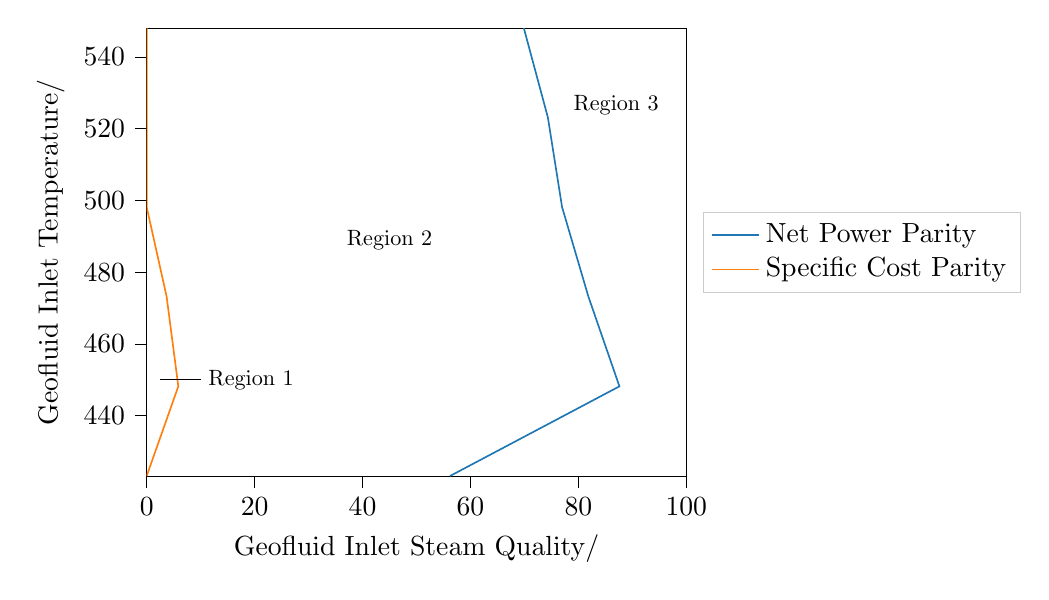
\begin{tikzpicture}

\definecolor{darkgray176}{RGB}{176,176,176}
\definecolor{darkorange25512714}{RGB}{255,127,14}
\definecolor{lightgray204}{RGB}{204,204,204}
\definecolor{steelblue31119180}{RGB}{31,119,180}

\begin{axis}[
legend cell align={left},
legend style={
  fill opacity=0.8,
  draw opacity=1,
  text opacity=1,
  at={(1.03,0.5)},
  anchor=west,
  draw=lightgray204
},
tick align=outside,
tick pos=left,
x grid style={darkgray176},
xlabel={Geofluid Inlet Steam Quality/\unit{\percent}},
xmin=0, xmax=100,
xtick style={color=black},
y grid style={darkgray176},
ylabel={Geofluid Inlet Temperature/\unit{\K}},
ymin=423, ymax=548,
ytick style={color=black}
]
\addplot [semithick, steelblue31119180]
table {%
56.211897840536 423.15
87.6035000467854 448.15
81.8582827723205 473.15
76.9746128225413 498.15
74.343495146738 523.15
69.870082455215 548.15
};
\addlegendentry{Net Power Parity}
\addplot [semithick, darkorange25512714]
table {%
0 423.15
5.86239070301085 448.15
3.70072396216428 473.15
0 498.15
0 523.15
0 548.15
};
\addlegendentry{Specific Cost Parity}
\draw (axis cs:87,525) node[
  scale=0.8,
  anchor=base,
  text=black,
  rotate=0.0
]{Region 3};
\draw (axis cs:45,487.5) node[
  scale=0.8,
  anchor=base,
  text=black,
  rotate=0.0
]{Region 2};
\draw[-,draw=black] (axis cs:10,450) -- (axis cs:2.5,450);
\draw (axis cs:10,450) node[
  scale=0.8,
  anchor=west,
  text=black,
  rotate=0.0
]{Region 1};
\end{axis}

\end{tikzpicture}
